\subsection{Internal Hardware Components of a computer} \noindent
  \marginnote{4.7.1.1} There are several component that lie within a computer, the main internal components are:
  \begin{itemize}
    \setlength{\itemsep}{0em}
    \item Processor
      \subitem A device that carries out computation on data by following instructions, in order to produce an output.
    \item Main Memory
      \subitem This stores data and instructions that will be used by processor.
    \item Address Bus
      \subitem A mono-directional (from processor to memory) bus that is used to specify a physical address in memory so that the data bus can access it.
    \item Data Bus
      \subitem This is a bi-directional bus that transfers data between the processor and memory.
    \item Control Bus
      \subitem This is a bi-directional bus that sends control signals to the registers, the data, and the address buses.
    \item I/O Controllers
      \subitem These control the flow of information between the processor and the input and output devices.
  \end{itemize}
  There are two main architectures you need to know about:
  \begin{itemize}
    \setlength{\itemsep}{0em}
    \item Von Neumann Architecture
      \subitem A technique for building a processor where data and instructions are stored in the same memory and accessed via buses This is used for common computing devices, e.g. a computer.\\
      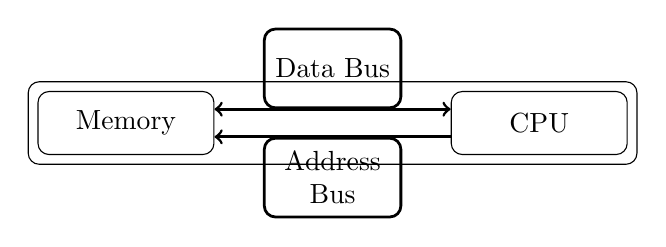
\begin{tikzpicture}
        \matrix[column sep=30mm]{
          \node[draw, minimum width=20mm,align=center, text width=20mm, minimum height=8mm] (Mem) {Memory}; & \node[draw, minimum width=20mm, align=center, text width=20mm, minimum height=8mm] (CPU) {CPU}; \\
        };
        \draw[<->, line width=1pt] ([yshift=5pt]Mem.east) -- node[above] {Data Bus} ([yshift=5pt]CPU.west);
        \draw[<-, line width=1pt] ([yshift=-5pt]Mem.east) -- node[below] {Address Bus} ([yshift=-5pt]CPU.west);
      \end{tikzpicture}
    \item Harvard Architecture
      \subitem A technique for building a processor that uses separate buses and memory for data and instructions. These are mainly used in embedded computer systems (e.g. mobile phones, burglar alarms, etc.) as data and instructions don't have to run down the same bus, meaning faster executions of programs.\\
      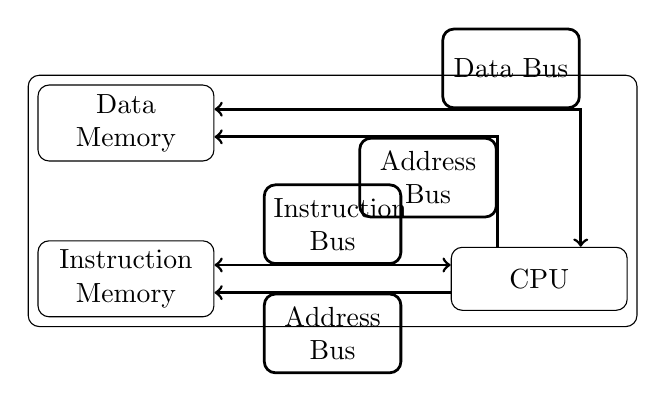
\begin{tikzpicture}
      \matrix[column sep=30mm, row sep=10mm]{
        \node[draw, minimum width=20mm,align=center, text width=20mm, minimum height=8mm] (Mem2) {Data Memory}; & \\
        \node[draw, minimum width=20mm,align=center, text width=20mm, minimum height=8mm] (Mem1) {Instruction Memory}; & \node[draw, minimum width=20mm, align=center, text width=20mm, minimum height=8mm] (CPU) {CPU}; \\
      };
      \draw[<->, line width=1pt] ([yshift=5pt]Mem1.east) -- node[above] {Instruction Bus} ([yshift=5pt]CPU.west);
      \draw[<-, line width=1pt] ([yshift=-5pt]Mem1.east) -- node[below] {Address Bus} ([yshift=-5pt]CPU.west);
      \draw[<->, line width=1pt] ([yshift=5pt]Mem2.east) -| node[above left] {Data Bus} ([xshift=15pt]CPU.north);
      \draw[<-, line width=1pt] ([yshift=-5pt]Mem2.east) -| node[below left] {Address Bus} ([xshift=-15pt]CPU.north);
      \end{tikzpicture}
  \end{itemize}
  Addressable memory is the concept that memory is made up of millions addressable cells with each cell being given a uniquely identifiable address, allowing programs and files to be stored across a number of these cells. The systematic way in which memory is organised allows different programs to be stored in different parts of the memory. A memory map could be made to show what type of programs are stored in what part of the memory.
\subsection{The Stored Program Concept} \noindent
  \marginnote{4.7.2.1}This is the concept that instructions and data are stored together in memory, and the instructions are fetched and executed serially by a processor that performs arithmetic and logical operations.
\subsection{Structure and Role of the Processor and its Components} \noindent
  \marginnote{4.7.3.1}There are many parts within the processor, the major components are:
  \begin{itemize}
    \setlength{\itemsep}{0em}
    \item Arithmetic Logic Unit (ALU)
      \subitem This is the part of the processor that processes and manipulates data. It can do two different types of operations, arithmetic and logical.
    \item Control Unit
      \subitem This is the part of the processor that manages the execution of instructions in the fetch-execute cycle.
    \item Clock
      \subitem This is a device that generated a signal used to synchronise the components of a computer. clock speed is measured in megahertz (MHz) or gigahertz(GHz) and shows how many pulses are sent per second.
    \item General-Purpose registers
      \subitem A small section of temporary storage that is part of the processor. Stores data or control instructions during fetch-decode-execute cycle.
    \item Dedicated Registers, including:
    \begin{itemize}
      \setlength{\itemsep}{0em}
      \item Program Counter (PC)
        \subitem This is a register that stores the address of the next instruction to be taken from main memory into the processor.
      \item Current Instruction Register (CIR)
        \subitem This is a register that stores the instructions that the CPU is currently decoding/ executing.
      \item Memory Address Register (MAR)
        \subitem This register stores the location of the address that data is either written to or copied from by the processor.
      \item Memory Buffer Register (MBR)
        \subitem This register holds data that is either written to or copied from the CPU.
      \item Status Register
        \subitem This keeps track of the various functions of the computer such as if the result of the last calculation was positive or negative.
    \end{itemize}
  \end{itemize}
  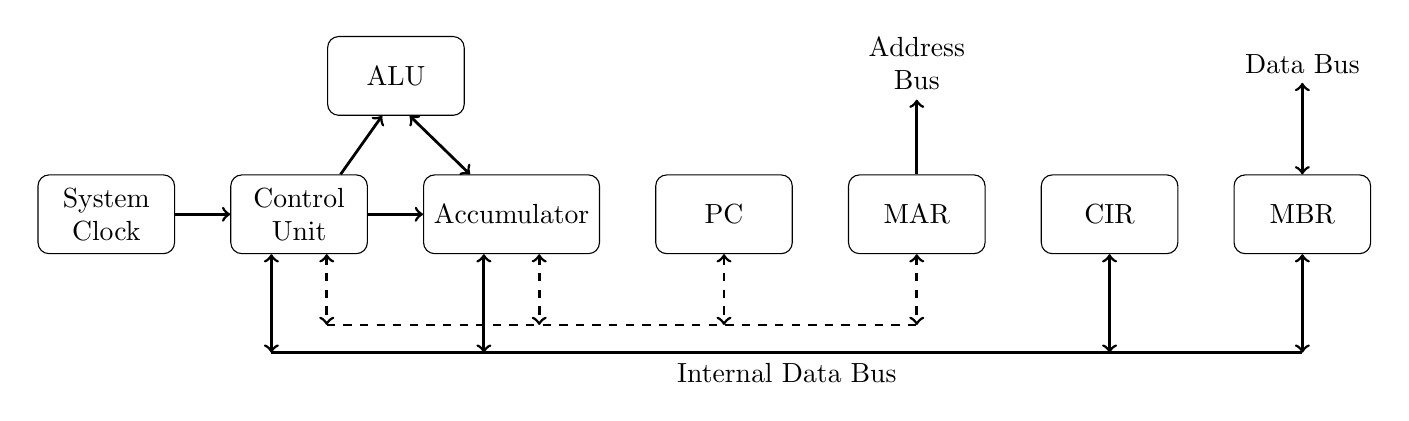
\begin{tikzpicture}
  \tikzstyle{every node}=[rectangle, rounded corners, text width=1.5cm,  minimum width=1.5cm, minimum height=1cm,text centered, draw=black]
    \matrix[column sep=7mm, draw=white]
    {
      \node (SC){System Clock}; &
      \node (CU){Control Unit}; &
      \node[text width=2cm,  minimum width=2cm] (A){Accumulator}; &
      \node (PC){PC}; &
      \node (MAR){MAR}; &
      \node (CIR){CIR}; &
      \node (MBR){MBR};
       \\
    };
    \node (ALU) at ([yshift=50pt, xshift=35pt]CU){ALU};
    \node[draw=white, minimum width=0cm, minimum height=0cm, text width=0cm] (B1) at ([yshift=-40pt]CU){};
    \node[draw=white, minimum width=0cm, minimum height=0cm, text width=0cm] (B2) at ([yshift=-50pt]CU){};
    \draw[->, line width=1pt] (SC.east) -- (CU.west);
    \draw[->, line width=1pt] (CU.east) -- (A.west);
    \draw[<->, line width=1pt] ([xshift=-10pt]CU.south) -- ( [xshift=-10pt]CU.south |- B2);
    \draw[<->, line width=1pt] ([xshift=-10pt]A.south) -- ( [xshift=-10pt]A.south |- B2);
    \draw[<->, line width=1pt] (CIR.south) -- (CIR.south |- B2);
    \draw[<->, line width=1pt] (MBR.south) -- ( MBR.south |- B2);
    \draw[line width=1pt] ( [xshift=-10pt]CU.south |- B2) -- node[below, opacity=0, text opacity=1, text width=5cm, minimum width=0cm, minimum height=0cm]{Internal Data Bus} (MBR.south |- B2);
    \draw[<->, line width=1pt, dashed] ([xshift=10pt]CU.south) -- ( [xshift=10pt]CU.south |- B1);
    \draw[<->, line width=1pt, dashed] ([xshift=10pt]A.south) -- ( [xshift=10pt]A.south |- B1);
    \draw[<->, line width=1pt, dashed] (PC.south) -- (PC.south |- B1);
    \draw[<->, line width=1pt, dashed] (MAR.south) -- (MAR.south |- B1);
    \draw[line width=1pt, dashed] ([xshift=10pt]CU.south |- B1) -- (MAR.south |- B1);
    \draw[->, line width=1pt] ([xshift=15pt]CU.north) -- ([xshift=-5pt]ALU.south);
    \draw[<->, line width=1pt] ([xshift=-15pt]A.north) -- ([xshift=5pt]ALU.south);
    \node[draw=white, minimum width=0cm, minimum height=0cm] (AB) at ([yshift=40pt]MAR.north) {Address Bus};
    \node[draw=white, minimum width=0cm, minimum height=0cm] (DB) at ([yshift=40pt]MBR.north) {Data Bus};
    \draw[->, line width=1pt] (MAR.north) -- (AB.south);
    \draw[<->, line width=1pt] (MBR.north) -- (DB.south);
  \end{tikzpicture}
  \marginnote{4.7.3.2}There are three steps for the Fetch-execute cycle
  \begin{enumerate}
    \item Fetch
      \subitem The program counter holds the address for the next instruction. The proceeor sends this address along the address bus to the main memory. The contents of the memory location at that address are sent via the data bus to the current instruction register and the program counter is incremented. The details of the addresses are initially loaded into the memory address register and the data initially goes to the memory buffer register. Some instructions need to load a number of bytes or words, so they may need to be fetched as successive parts of a single instruction.
    \item Decode
      \subitem The processor then takes the instruction from the CIR and decides what to do with it. It does this by referring to the instruction set. These instruction sets are either classed as an RISC (Reduced Instruction Set) or CISC (Complex Instruction Set). An instruction set is a library of all the things the processor can be asked to do. Each instruction in the instruction set is accompanied by details of what the processor should do when it receives that particular instruction. This might be to send the contents of the memory buffer register to the arithmetic logic unit.
    \item Execute
      \subitem Once the instruction that has just been taken from the memory has been decoded, the processor now carries out the instruction. It then goes back to the top of the cycle and fetches the next instruction. A simple instruction will require only a single clock cycle, whereas a complex instruction may need three or four. The results of any calculations are written either to a register or a memory location.
  \end{enumerate}
  \marginnote{4.7.3.3}An instruction set is a set of instructions that a processor can perform written in machine code, each processor has its own unique instruction set. A simple instruction can be split into three different parts:
  \begin{itemize}
    \item Opcode
      \subitem an operation code or instructions used in assembly language.
    \item Operand
      \subitem a value or memory address that forms part of an assembly language instructions. The number of operands a needed depends on the opcode being used.
    \item Addressing Mode
      \subitem The way in which the operand is interpreted (a memory address or an actual value)
  \end{itemize}
  Here's an example of a possible instruction using a 32 bit scheme (the precise format is up to the designer of the processor, the following uses 16 bits for the op code, 4 bits for the addressing code, and 12 bits for the operand):
  \(\underbrace{1101010011101000}_{\text{Opcode}}\underbrace{0001}_{\text{Adressing Mode}}\underbrace{010011110011}_{\text{Operand}}\) \\
  \marginnote{4.7.3.4}There are two main types of addressing modes:
  \begin{itemize}
    \item Direct addressing
      \subitem This means that the operand refers to the address of the datum, meaning that the data is held in RAM or in a register, and the operand says where to find the data.
    \item Immediate addressing
      \subitem This means the operand is the datum, so for example \#10 would mean immediate address and that the value to use is the number 10.
  \end{itemize}
  \marginnote{4.7.3.5}There are a large array of opcodes, here are the ones you will need to know:
  \begin{itemize}
    \setlength{\itemsep}{0em}
    \item Load
      \subitem This loads the value stored in the memory location specified by \verb|<memory ref>| into register \verb|d|: \verb|LDR Rd, <memory ref>|
    \item Add
      \subitem Add the value specified in \verb|<operand2>| to the value in register \verb|n| and store the result in register \verb|d|: \verb|ADD Rd, Rn, <Operand2>|
    \item Subtract
      \subitem Subtract the value specified in \verb|<operand2>| to the value in register \verb|n| and store the result in register \verb|d|: \verb|SUB Rd, Rn, <Operand2>|
    \item Store
      \subitem Store the value that is in register \verb|d| into the memory location specified by \verb|<memory ref>|: \verb|STR Rd, <memory ref>|
    \item Branching
    \begin{itemize}
      \setlength{\itemsep}{0em}
      \item Conditional
        \subitem Conditionally branch to the instruction at position \verb|<label>| in the program if the last comparison met the criteria specified by the \verb|<condition>|. Possible values for \verb|<condition>| and their meanings are: \verb|EQ|-Equal to, \verb|NE|-Not equal to, \verb|GT|-Greater than, \verb|LT|-Later than: \verb|B<condition> <label>|
      \item Unconditional
        \subitem Always branch to the instruction at position \verb|<label>| in the program: \verb|B <label>|
    \end{itemize}
    \item Compare
      \subitem Compare the value stored in register \verb|n| with the value specified by \verb|<operand2>|: \verb|CMP Rn, <operand2>|
    \item Logical Bitwise Operators
    \begin{itemize}
      \setlength{\itemsep}{0em}
      \item AND
        \subitem Perform a bitwise logical AND operation between the value in register \verb|n| and the value specified by \verb|<operand2>| and store the result in register \verb|d|: \verb|AND Rd, Rn, <operand2>|
      \item OR
        \subitem Perform a bitwise logical OR operation between the value in register \verb|n| and the value specified by \verb|<operand2>| and store the result in register \verb|d|: \verb|ORR Rd, Rn, <operand2>|
      \item NOT
        \subitem Perform a bitwise logical NOT on the value specified by \verb|<operand2>| and store the result in register \verb|d|: \verb|MVN Rd, <operand2>|
      \item XOR
        \subitem Perform a bitwise logical XOR operation between the value in register \verb|n| and the value specified by \verb|<operand2>| and store the result in register \verb|d|: \verb|EOR Rd, Rn, <operand2>|
    \end{itemize}
    \item Logical
    \begin{itemize}
      \setlength{\itemsep}{0em}
      \item Shift Left
        \subitem Logically shift left the value stored in register \verb|n| by the number of bits specified by \verb|<operand2>| and store the result in register \verb|d|: \verb|LSL Rd, Rn, <operand2>|
      \item Shift Right
        \subitem Logically shift right the value stored in register \verb|n| by the number of bits specified by \verb|<operand2>| and store the result in register \verb|d|: \verb|LSR Rd, Rn, <operand2>|
    \end{itemize}
    \item Halt
      \subitem Stops the execution of the program.
  \end{itemize}
  \marginnote{4.7.3.6}Interrupts
  
  \noindent
  \marginnote{4.7.3.7}There are several factors that can impact the performance of a processor:
  \begin{itemize}
    \setlength{\itemsep}{0em}
    \item Multiple Cores
      \subitem Multiple cores means that multiple instructions can be carried out at once, so more processsors can lead to an increase in processor performance.
    \item Cache Memory
      \subitem This involves a technique where instructions and data that are frequently used are stored in cache memory (a high-speed temporary area of memory), so programs run faster.
    \item Clock Speed
      \subitem This indicates how many pulses the clock sends out per second and thus indicates the maximum number of instructions that can be performed per second, so increasing clock speed may increase processor performance.
    \item Word Length
      \subitem This indicates the number of bits the can be addressed, transferred or manipulated as one unit. Increasing the word length means that more data can be processed at each pulse of the unit clock.
    \item Address Bus Width
      \subitem This indicates the number of bits that can be sent down the address bus in one go (during one clock pulse), increasing the address bus width means more memory can be addressed, so more memory can be installed on the computer.
    \item Data Bus Width
      \subitem This indicates the number of bits that can be sent down the data bus in one go (during one clock pulse), increasing the data bus width means more data can be sent down the bus during each clock pulse, so more data can be processed within a given time.
  \end{itemize}
\subsection{External Hardware Devices}
  \noindent
  \marginnote{4.7.4.1}We need to know the purpose and principles of operation for 4 I/O devices:
  \begin{itemize}
    \setlength{\itemsep}{0em}
    \item Barcode Reader
      \subitem Barcodes are used primarily for inputting product details at the point of sale. This can be done by passing the object over a scanner or by using a handheld scanner to scan the barcode. They work in the following way:
      \begin{enumerate}
        \setlength{\itemsep}{0em}
        \item A light (an LED or laser) is passed over an image
        \item Some form of light sensor is used to measure the intensity of light that is reflected which is converted into a current, effectively generating a waveform by using a photodiode or charge coupled device (CCD).
        \item white areas reflect the most light whereas black reflects the least, so the waveform can be used to identify the pattern of black and white bars.
        \item The analogue waveform needs to be converted into digital form using and ADC, encoding the white and black into binary (for example, black=0, white=1).
        \item The signal is decoded into a form that can be interpreted by software.
      \end{enumerate}
    \item Digital Camera
      \subitem Digital Camera's are useful for creating digital images of photographs, which can then be printed ir transferred onto a computer to be manipulated and stored. The quality of a camera is dictated by how many pixels it uses to record the image, e.g. a 12 megapixel camera stores data on 12,000,000 pixels. They work in the following way:
      \begin{enumerate}
        \setlength{\itemsep}{0em}
        \item When a photograph is taken the shutter opens and lets light in through the lens.
        \item The light is focused onto a sensor (charge coupled device (CCD) or a complementary metal oxide semiconductor (CMOS)).
        \item The sensors are made up of millions of transistors, each of which stores the data for one or more pixels.
        \item As the light hits the sensors, it is converted into electrons and the amount of charge is recorded for each pixel in digital form.
        \item With light, all colours can be created from red, green and blue (RGB). Therefore to record colour, the camera will either have three different sensors, or use three different sensors, one for each colour.
        \item The data are typically stored on removable storage devices, usually referred to as flash memory, which uses programmable ROM and are usually stored in compressed files, e.g. TIFF, JPEG or PNG. (Raw files can also be generated, which are uncompressed and therefore contain all of the data from the original paragraph)
        \item This digital data can now be decoded and manipulated using specialised software.
      \end{enumerate}
    \item Laser Printer
      \subitem This is a device that uses lasers and toner to create mono and colour prints, its major advantage over standard home printers is that it is much faster, and is built to print many different documents. it works in the following way:
      \begin{enumerate}
        \setlength{\itemsep}{0em}
        \item A rotating drum inside the printer is coated in a chemical which holds an electrical charge.
        \item The laser beam is reflected by a mirror onto the drum and where the light hits the drum the charge is discharged, effectively creating the image on the drum.
        \item As the drum rotates it picks up toner which is attracted to the charged part of the drum.
          \subitem If printing in colour, then four colours will need to be used: cyan, yellow, magenta, and key (black) (CMYK), so either the paper has to go around the drum 4 times, or a transfer belt may be used to hold all of the colours.
        \item Paper is passed over the drum and by charging the paper with the opposite charge to the toner, the toner is attracted to the paper and away from the drum. The paper is heat treated to fuse the toner onto the paper.
      \end{enumerate}
    \item Radio Frequency Identification (RFID)
      \subitem This is a microscopic device that stores data and transmits it using radio waves - usually used in tags to track items. It works in the following way:
      \begin{itemize}
        \setlength{\itemsep}{0em}
        \item The tag contains a chip, which contains data about the item and a modem to modulate and demodulate the radio signals, it also contains an antennae to send and receive signals.
        \item Tags can be either active, meaning they have their own power supply or passive, meaning that they will pick up electromagnetic power when they are in range of a RFID reader.
        \item Signals, and therefore data, can be transmitted in both directions using radio frequencies. This may be over a short or long distance depending on how the tag is built. The typical range is between 1 and 100m.
        \item Tags may be used to simply track the physical location of an item or the data may transmit data back.
      \end{itemize}
      \subitem RFID is a relatively new tech and it is being put to various uses, some of which are controversial. Applications include:
      \begin{itemize}
        \item Tracking individuals, particularly vulnerable adults such as Alzheimer's patients.
        \item Use in electronic passports to keep track of where people travel.
        \item Tags have been added to credit and debit cards allow users to make contactless payment via RFID in a shop.
        \item Transport and distribution companies can use RFID to track shipments and deliveries
        \item Tags have been added to high value items, for example artworks in museums or equipment in hospitals.
      \end{itemize}
  \end{itemize}
  \marginnote{4.7.4.2}Secondary storage devices are used within computers to allow data to be permanently stored within it. There are three main secondary storage devices:
  \begin{itemize}
    \setlength{\itemsep}{0em}
    \item Hard Disk (HDD)
      \subitem Hard disks are constructed of hard metallic material and are hermetically sealed (air-tight). This is to protect them from being corrupted by dust or other debris. Most hard disks are in fact made up of a number of disks arranged in a stack. The disks are coated with a thin film of magnetic material. Changes in direction of magnetism represents zeros and ones.
      \begin{itemize}
        \item hard disks spin at speeds between 3600 and 12500 RPM, as a series of heads read from and write to the disks.
        \item The heads do not actually touch the surface of the disk but float slightly above it by virtue of the speed at which the disk spins.
        \item There is an actuator arm which moves the head across the surface of the disk as it spins.
        \item The combination of the rotating of the disks with lateral movement of the arm means that the head can access every part of the disk surface.
        \item The surface of the disk is organised into concentric tracks and each track is split into sectors each of which can be addressed by the OS.
        \item Because all of the actuator arms move at the same time due to the assembly head, the cylinder is often referenced, which simply just says what track the data is on for all of the disks.
        \item Each sector has the same capacity and a large file will be stored over a number of sectors.
        \item The OS groups sectors together into clusters to make storage easier to manage, there will be many occasions when a whole cluster is not needed, leading to redundant space.
          \subitem For example, a file may need four sectors and part of the fifth, so it will be allocated all 5 sectors, meaning there's empty (redundant) space that can't be used.
      \end{itemize}
    \item Optical Disk
      \subitem Optical disk is a generic term for all variations of CD, DVD and Blu-Ray that use laser technology to read and write data. An optical disk is made up of one single spiral track that starts in the middle and work it's way to the edge of the CD. The laser will read data that are contained within this track by reading the pits (lower parts) and lands (higher parts) in combination with a sensor that measures how much light is reflected.
      \begin{itemize}
        \item For read-only optical disks, when data is written it is encoded as a series of pits and lands within the track of the disk.
        \item A protective layer is then put over the surface to prevent any data corruption, the pattern of pits and lands are used to represent data.
        \item When the CD is read, the pits and lands are read by the laser which then interprets each as different electrical signals, then the electrical signals can be converted into binary codes.
          \subitem
        \item For writeable optical disks, rather than using pits and lands, the disk is coated photosensitive dye, which is translucent, when writing to the disk, the laser will alter the state of a dye spot that is coated onto the surface making it opaque.
        \item The dye reflects a certain amount of light.
        \item A write laser alters the density of the dye and a read laser interprets the different densities to create binary patterns which in turn can represent data, write lasers are higher powered than read lasers.
      \end{itemize}
    \item Solid-State Disk (SSD)
      \subitem Solid-state disks use programmable ROM chips, similar to memory cards, hence they are more often referred to as Solid-state drive instead of solid-state disk.
      \begin{itemize}
        \item These are stored inside a unit that looks like a hard disk and commonly uses a type of memory called NAND memory.
        \item This organises data into blocks in a similar way to traditional hard disk as described earlier, with a controller being used to manage the blocks of data.
        \item Blocks of a set physical size will be made up of binary data.
        \item When reading and writing, data can only be accessed in blocks.
        \item With SSD, blocks will be allocated to particular semiconductors, meaning data can be added and deleted to different blocks to different areas of the drive, sso that only small parts of the drive have to be erased and written to, enabling very fast access times.
        \item It uses a floating gate transistor to be able to trap and store charge, it contains two gates: floating gate and control gate, a thin layer of oxide is placed between the two gates, trapping the charge inside the floating gate even when power is turned off.
      \end{itemize}
  \end{itemize}
  Here is a table comparing the different devices:
  \begin{table}[H]
    \centering
    \begin{tabular}{ L{3cm} | L{2.5cm} | L{3.5cm} | L{3cm} | L{3cm} }
       & \textbf{Hard Disk (HDD)} & \textbf{Solid State Disk (SDD)} & \textbf{Optical Disk (CD/DVD)} & \textbf{Optical Disk (Blu-ray)} \\ \hline
       \textbf{Typical Capacity} & High (1 TB) & Medium (500 GB) & Low (900 MB to 1.7 GB) & Low to Medium (25-50 GB) \\ \hline
       \textbf{Relative Cost} & Medium & High & Low & Low \\ \hline
       \textbf{Easily portable} & External disks are available & External disks are available & Yes & Yes \\ \hline
       \textbf{Relative Power Consumption} & High & Low & High & High \\ \hline
       \textbf{Relative Speed of access} & Medium & High & Low & Low \\ \hline
       \textbf{Latency} & High & Low & Very High & High \\ \hline
       \textbf{Fragmentation} & & None &  & \\ \hline
       \textbf{Reliability} & Good & Very Good & Fair & Fair \\ \hline
       \textbf{Relative Physical size} & Large & Small & Large & Large
    \end{tabular}
  \end{table}
